% ROBT613 midterm report. Compile on Overleaf (IEEEtran is bundled) or with pdflatex + bibtex.
% Every number comes from report/numbers.tex, generated by report/make_numbers.py from results/tables.
% Style rule for body text (PLAN.md 9): no colons or semicolons.
\documentclass[conference]{IEEEtran}
\usepackage{graphicx}
\usepackage{booktabs}
\usepackage{amsmath}
\usepackage{url}
\graphicspath{{figures/}}
% generated by report/make_numbers.py from results/tables -- do not edit
\newcommand{\NRecordings}{18}
\newcommand{\NTrialsSession}{288}
\newcommand{\NTrialsTotal}{5184}
\newcommand{\ExpertMin}{5}
\newcommand{\ExpertMax}{73}
\newcommand{\ExpertTotal}{488}
\newcommand{\ExpertPct}{9.4}
\newcommand{\CalibAFourT}{80}
\newcommand{\FilterTaps}{825}
\newcommand{\FilterLenS}{3.3}
\newcommand{\GainFiftyDefault}{-4.5}
\newcommand{\GainFifty}{-51}
\newcommand{\LineMax}{20}
\newcommand{\LineMaxRec}{S5 1test}
\newcommand{\IcaExclTwo}{17}
\newcommand{\IcaExclMax}{3}
\newcommand{\IcaMinScore}{0.55}
\newcommand{\FzEogRNone}{0.73}
\newcommand{\FzEogRReg}{0.08}
\newcommand{\FzEogRIca}{0.15}
\newcommand{\PtpMax}{142}
\newcommand{\PtpPctNineNineFive}{107}
\newcommand{\RegInjected}{6}
\newcommand{\RegInjectedExpert}{6}
\newcommand{\RegInjectedMax}{395}
\newcommand{\HeogPos}{17}
\newcommand{\HeogSig}{15}
\newcommand{\HeogDMax}{3.24}
\newcommand{\HeogOnsetMin}{192}
\newcommand{\HeogOnsetMax}{196}
\newcommand{\HeogPeak}{366}
\newcommand{\LatNegAny}{18}
\newcommand{\LatNegBeta}{18}
\newcommand{\WeakErd}{S2 0train, S5 0train, S5 1test, S7 0train}
\newcommand{\SNineHighP}{1.6e-19}
\newcommand{\AucEogNoneT}{0.86}
\newcommand{\AboveEogNoneT}{8}
\newcommand{\AucAllNoneT}{0.85}
\newcommand{\AboveAllNoneT}{8}
\newcommand{\AucAllRegT}{0.83}
\newcommand{\AboveAllRegT}{8}
\newcommand{\AucAllIcaT}{0.80}
\newcommand{\AboveAllIcaT}{8}
\newcommand{\AucPhysioNoneT}{0.77}
\newcommand{\AbovePhysioNoneT}{8}
\newcommand{\AucPhysioRegT}{0.77}
\newcommand{\AbovePhysioRegT}{8}
\newcommand{\AucPhysioIcaT}{0.77}
\newcommand{\AbovePhysioIcaT}{8}
\newcommand{\AucProneNoneT}{0.57}
\newcommand{\AboveProneNoneT}{3}
\newcommand{\AucProneRegT}{0.58}
\newcommand{\AboveProneRegT}{3}
\newcommand{\AucProneIcaT}{0.56}
\newcommand{\AboveProneIcaT}{3}
\newcommand{\AucEogNoneE}{0.87}
\newcommand{\AboveEogNoneE}{9}
\newcommand{\AucAllNoneE}{0.86}
\newcommand{\AboveAllNoneE}{8}
\newcommand{\AucAllRegE}{0.83}
\newcommand{\AboveAllRegE}{7}
\newcommand{\AucAllIcaE}{0.89}
\newcommand{\AboveAllIcaE}{8}
\newcommand{\AucPhysioNoneE}{0.80}
\newcommand{\AbovePhysioNoneE}{8}
\newcommand{\AucPhysioRegE}{0.80}
\newcommand{\AbovePhysioRegE}{9}
\newcommand{\AucPhysioIcaE}{0.87}
\newcommand{\AbovePhysioIcaE}{7}
\newcommand{\AucProneNoneE}{0.59}
\newcommand{\AboveProneNoneE}{3}
\newcommand{\AucProneRegE}{0.53}
\newcommand{\AboveProneRegE}{2}
\newcommand{\AucProneIcaE}{0.54}
\newcommand{\AboveProneIcaE}{4}
\newcommand{\BaccEogNone}{0.56}
\newcommand{\BaccAllNone}{0.59}
\newcommand{\BaccAllIca}{0.58}
\newcommand{\BaccPhysioNone}{0.59}
\newcommand{\BaccPhysioIca}{0.64}
\newcommand{\BaccProneNone}{0.34}
\newcommand{\BaccProneIca}{0.32}
\newcommand{\BaccChance}{0.29}
\newcommand{\NestedDiff}{0.007}
\newcommand{\XsEog}{0.84}
\newcommand{\XsAllNone}{0.86}
\newcommand{\XsAllIca}{0.89}
\newcommand{\HoneP}{0.002}
\newcommand{\HoneW}{45}
\newcommand{\HoneDelta}{0.36}
\newcommand{\HoneIqrLo}{0.27}
\newcommand{\HoneIqrHi}{0.47}
\newcommand{\HoneAbove}{8}
\newcommand{\HoneN}{9}
\newcommand{\HoneVerdict}{supported}
\newcommand{\HtwoPReg}{0.633}
\newcommand{\HtwoPholmReg}{1.000}
\newcommand{\HtwoDeltaReg}{-0.002}
\newcommand{\HtwoRhoReg}{0.35}
\newcommand{\HtwoRhoPReg}{0.356}
\newcommand{\HtwoPIca}{0.633}
\newcommand{\HtwoPholmIca}{1.000}
\newcommand{\HtwoDeltaIca}{-0.002}
\newcommand{\HtwoRhoIca}{-0.42}
\newcommand{\HtwoRhoPIca}{0.265}
\newcommand{\HtwoVerdict}{not supported}
\newcommand{\HthreeP}{0.752}
\newcommand{\HthreeDropPhysio}{-0.010}
\newcommand{\HthreeDropProne}{-0.057}
\newcommand{\HthreeShareNone}{24.8}
\newcommand{\HthreeShareIca}{27.6}
\newcommand{\HthreeShareP}{0.125}
\newcommand{\HthreeVerdict}{not supported}
\newcommand{\RobHoneAll}{all}
\newcommand{\RobHoneN}{5}
\newcommand{\RobHtwoAny}{0}
\newcommand{\RobHtwoN}{10}
\newcommand{\ExPReg}{0.125}
\newcommand{\ExPholmReg}{0.375}
\newcommand{\ExAucReg}{0.67}
\newcommand{\ExDeltaReg}{0.013}
\newcommand{\ExRhoReg}{0.98}
\newcommand{\ExRhoPReg}{1.9e-06}
\newcommand{\ExPIca}{0.590}
\newcommand{\ExPholmIca}{0.652}
\newcommand{\ExAucIca}{0.71}
\newcommand{\ExDeltaIca}{-0.025}
\newcommand{\ExRhoIca}{0.85}
\newcommand{\ExRhoPIca}{0.004}
\newcommand{\ExAucNone}{0.70}
\newcommand{\ExAboveNone}{8}
\newcommand{\TimeDecode}{6.2}
\newcommand{\NPermH}{100}


\begin{document}

\title{Eye Movements Decode Motor Imagery in BCI Competition IV 2a,\\ but Band-Power EEG Decoders Do Not Depend on Them}

\author{\IEEEauthorblockN{Chidiadi Bethel Mba, Sungkar Bolat, Beibars Ybraiakhyn, Ramazan Zypayev}
\IEEEauthorblockA{ROBT613 Brain Machine Interface, Nazarbayev University}}

\maketitle

\begin{abstract}
The arrow cue of the most widely used motor-imagery (MI) benchmark, BCI Competition IV dataset 2a, points in the direction of the task. We asked how much of MI decoding on this dataset comes from ocular activity rather than sensorimotor rhythms. Three pre-registered hypotheses were tested on all 9 subjects with leave-one-run-out cross-validation and permutation chance levels. A decoder trained on the three EOG channels alone separated left from right hand imagery with a median ROC AUC of \AucEogNoneT{} (\HoneAbove{} of \HoneN{} subjects above their own permutation null, Wilcoxon $p=\HoneP{}$). The cue-locked horizontal EOG moved toward the cued side about \HeogPeak{}~ms after the cue in \HeogPos{} of \NRecordings{} recordings. Even so, removing ocular activity from the EEG with EOG regression or ICA, both fitted on separate calibration recordings, did not lower band-power EEG decoding (median change \HtwoDeltaIca{} AUC after ICA, $p=\HtwoPIca{}$). The decoder weights did not shift toward central channels in a measurable way. The confound is real and large, but it lives in the time domain. Band-power decoders restricted to the MI window do not pick it up in this dataset. In an exploratory time-domain decoder on frontal EEG the loss after cleaning grew with each subject's EOG-only AUC, which shows where the risk lies.
\end{abstract}

\section{Introduction}
Motor-imagery BCIs are meant for users who cannot move. A decoder that relies on eye or muscle activity may score well in the lab and then fail for exactly those users. EOG and EMG artifacts are the most common physiological artifacts in BCI work \cite{fatourechi2007}. Cranial EMG contaminates MI control during early training \cite{mcfarland2005} and its spectrum overlaps the beta band \cite{goncharova2003}. Dataset 2a of BCI Competition IV \cite{brunner2008,tangermann2012} is the most used MI benchmark. Its cue is an arrow pointing left, right, down or up for the four classes. The dataset description states that the EOG channels must not be used for classification and that artifacts should not influence the result \cite{brunner2008}. Whether they do has practical weight because results on 2a are compared across hundreds of papers.

We test three hypotheses that were written down before the full pipeline was run. H1 states that the EOG alone decodes left versus right hand above chance in most subjects. H2 states that removing ocular activity lowers EEG decoding, and more so in subjects with strong EOG decoding. H3 states that cleaning moves the discriminative weight from frontal channels and artifact-prone bands to central mu and beta features. All methods come from the ROBT613 workshop notebooks 00--06.

\section{Dataset and data audit}
Nine subjects performed cued left hand, right hand, feet and tongue imagery in two sessions on different days \cite{brunner2008}. Each session has 6 runs of 48 trials, giving \NTrialsSession{} trials per session and \NTrialsTotal{} in total. A fixation cross appears at $t=0$, the arrow at $t=2$~s for 1.25~s, and imagery lasts until $t=6$~s. EEG was recorded from 22 Ag/AgCl electrodes against the left mastoid and 3 monopolar EOG electrodes, at 250~Hz with a 0.5--100~Hz band-pass and a 50~Hz notch \cite{brunner2008}.

Data were loaded with MOABB 1.7.2 and every fact was checked against the loaded files (Table~\ref{tab:audit}). The MOABB annotation sits 2.0~s after the trial-start trigger, at cue onset, for every trial. The cue-locked EOG response confirms this independently (Section~\ref{sec:neuro}). MOABB drops two parts of the source files that this study needs. The expert artifact flags mark between \ExpertMin{} and \ExpertMax{} trials per session (\ExpertPct{}\% overall). The EOG calibration runs (eyes open, eyes closed, eye movements) are recorded at the start of each session. Both were read back from the cached source files. Subject A04T has a single calibration run of \CalibAFourT{}~s, as documented. EOG1 sits at the left outer canthus, EOG2 above the nasion and EOG3 at the right outer canthus (read from Fig.~3 of \cite{brunner2008}). We define HEOG as EOG1 minus EOG3 and VEOG as EOG2 minus the mean of EOG1 and EOG3.

\begin{table}[t]
\caption{Data audit (results/tables/audit\_summary.csv)}
\label{tab:audit}
\centering
\begin{tabular}{@{}ll@{}}
\toprule
Recordings & \NRecordings{} (9 subjects $\times$ 2 sessions)\\
Runs, trials per session & 6, \NTrialsSession{} (72 per class)\\
Channels & 22 EEG, 3 EOG, 250 Hz, Volts\\
Event marker & cue onset (verified)\\
Expert-flagged trials & \ExpertMin{}--\ExpertMax{} per session\\
\bottomrule
\end{tabular}
\end{table}

\section{Methods}
\subsection{Signal inspection and filtering}
Unfiltered spectra (Fig.~\ref{fig:psd}) show drift below 1~Hz in every recording and residual 50~Hz line noise up to \LineMax{}~dB above its flanks (\LineMaxRec{}) despite the notch applied at recording. We used a zero-phase FIR band-pass of 1--45~Hz (\FilterTaps{} taps, \FilterLenS{}~s). The 1~Hz edge removes drift and helps ICA. The upper transition band was set to 5~Hz. With the default transition the gain at 50~Hz is only \GainFiftyDefault{}~dB, while the chosen design gives \GainFifty{}~dB. A separate notch was therefore unnecessary. The data were not resampled.

\begin{figure}[t]
\centering
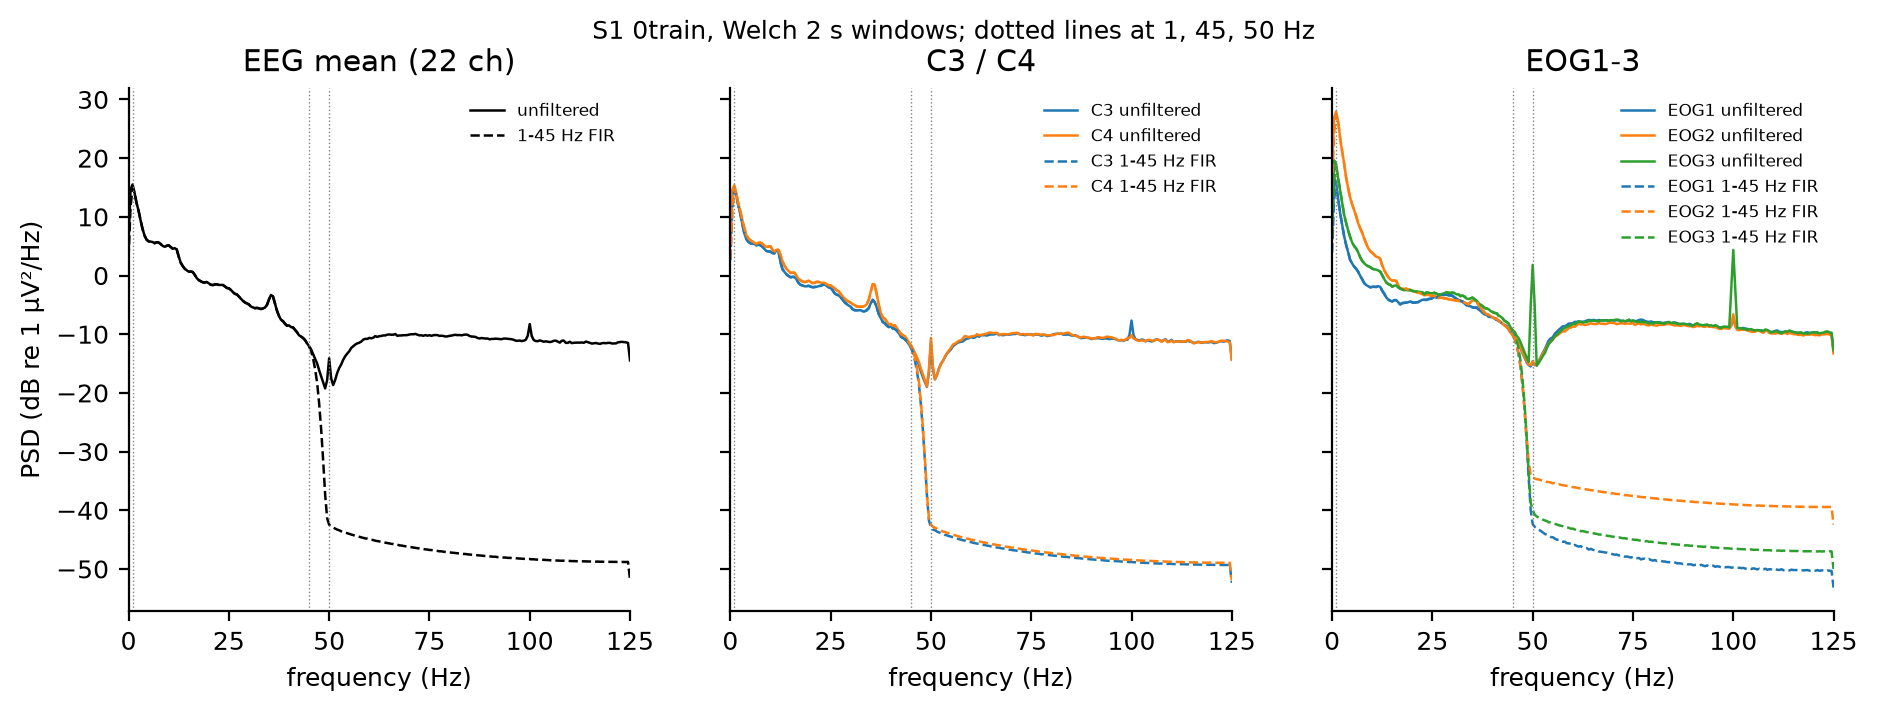
\includegraphics[width=\columnwidth]{fig_2a_psd_before_after.png}
\caption{Welch spectra of S1 before and after the 1--45~Hz filter.}
\label{fig:psd}
\end{figure}

\subsection{Artifact handling}
Three cleaning conditions share the same 288 epochs per recording. Condition \emph{none} is the filter followed by a common average reference (CAR). CAR was chosen because the recorded mastoid reference artificially lowers power at C5, next to the reference electrode, which would bias a left versus right comparison. Condition \emph{eog\_reg} adds least-squares regression of the three EOG channels out of every EEG channel. Condition \emph{ica} adds FastICA with 20 components (CAR leaves rank 21) and removes components whose time course correlates with any EOG channel at $|r|\ge0.5$. The distribution of this correlation over all 360 components has a gap between about 0.25 and 0.55, so the threshold does not cut through a cluster. Two components were removed in \IcaExclTwo{} recordings and at most \IcaExclMax{}.

Both cleaning models were fitted on the EOG calibration runs of the same session and then applied to the MI runs. No MI trial therefore enters any cleaning fit, in line with the course rule that a learned preprocessing step is fitted on calibration data. Cleaning worked on the held-out MI runs (Fig.~\ref{fig:clean}). The median absolute correlation between Fz and EOG2 fell from \FzEogRNone{} to \FzEogRReg{} after regression and \FzEogRIca{} after ICA.

No peak-to-peak rejection was applied. The largest epoch reached \PtpMax{}~$\mu$V (99.5th percentile \PtpPctNineNineFive{}~$\mu$V), so there were no gross outliers. A secondary mode of large epochs in \emph{none} shrinks after cleaning, so it is ocular, and rejecting it would remove the very trials under study. Regression has one failure mode. When an EOG electrode records a non-ocular step, regression copies it into the EEG. This raised \RegInjected{} epochs above the largest uncleaned value (up to \RegInjectedMax{}~$\mu$V), and all \RegInjectedExpert{} of them carry an expert artifact flag. A sensitivity analysis therefore repeats the tests without expert-flagged trials.

\begin{figure}[t]
\centering
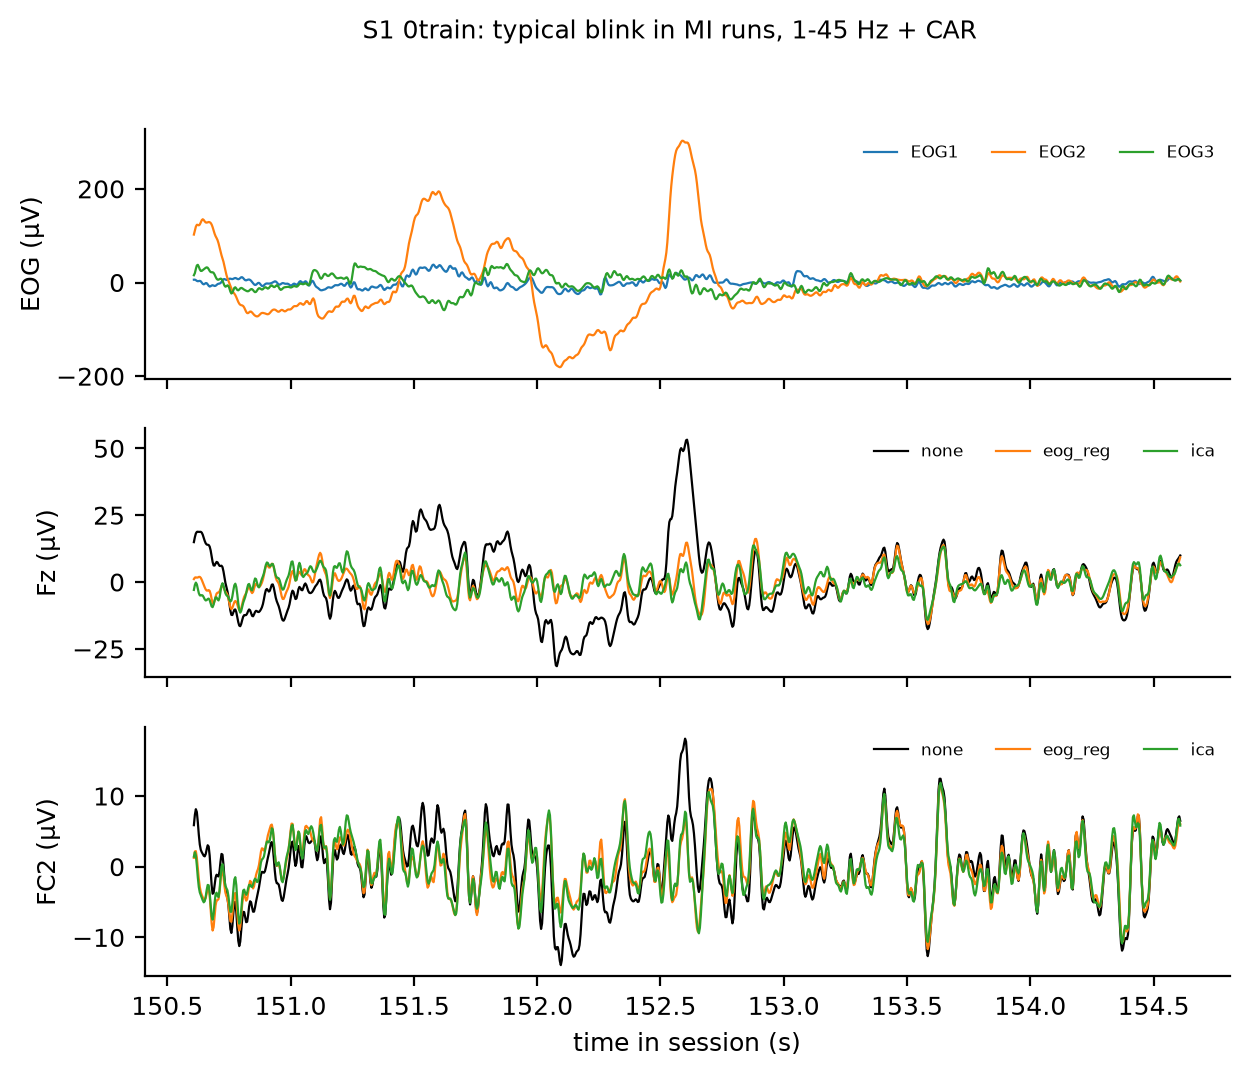
\includegraphics[width=\columnwidth]{fig_3b_eog_regression_before_after.png}
\caption{A blink and vertical eye movements in S1 leak into Fz and FC2 in \emph{none}. Both cleaning conditions remove them.}
\label{fig:clean}
\end{figure}

\subsection{Neurophysiological check}\label{sec:neuro}
Before any classifier was trained we checked that the expected signal and the suspected confound exist. Event-related desynchronisation (ERD) \cite{pfurtscheller1999} was computed as the change in log Welch band power between the fixation baseline ($-1$ to 0~s) and the MI window (0.5 to 2.5~s after the cue). Contralateral beta lateralisation was negative, as expected, in \LatNegBeta{} of \NRecordings{} recordings after ICA, while \WeakErd{} showed weak lateralisation (above $-0.5$~dB in both bands). These subjects were kept in the analysis.

The cue-locked HEOG separates left from right cues clearly (Fig.~\ref{fig:eog}). Left arrows drive the eyes to the left and right arrows to the right, and the up and down arrows of the tongue and feet classes produce matching VEOG deflections. The difference starts \HeogOnsetMin{}--\HeogOnsetMax{}~ms after the annotation and peaks at about \HeogPeak{}~ms, with no deflection before the cue. The mean HEOG between 0.2 and 1.0~s differs between left and right cues in the expected direction in \HeogPos{} of \NRecordings{} recordings, with $p<0.001$ in \HeogSig{} (Cohen's $d$ up to \HeogDMax{}). A return movement follows when the arrow disappears, inside the MI window. The same left versus right difference appears at FC3 and FC4 and is only partly removed by either cleaning method.

\begin{figure*}[t]
\centering
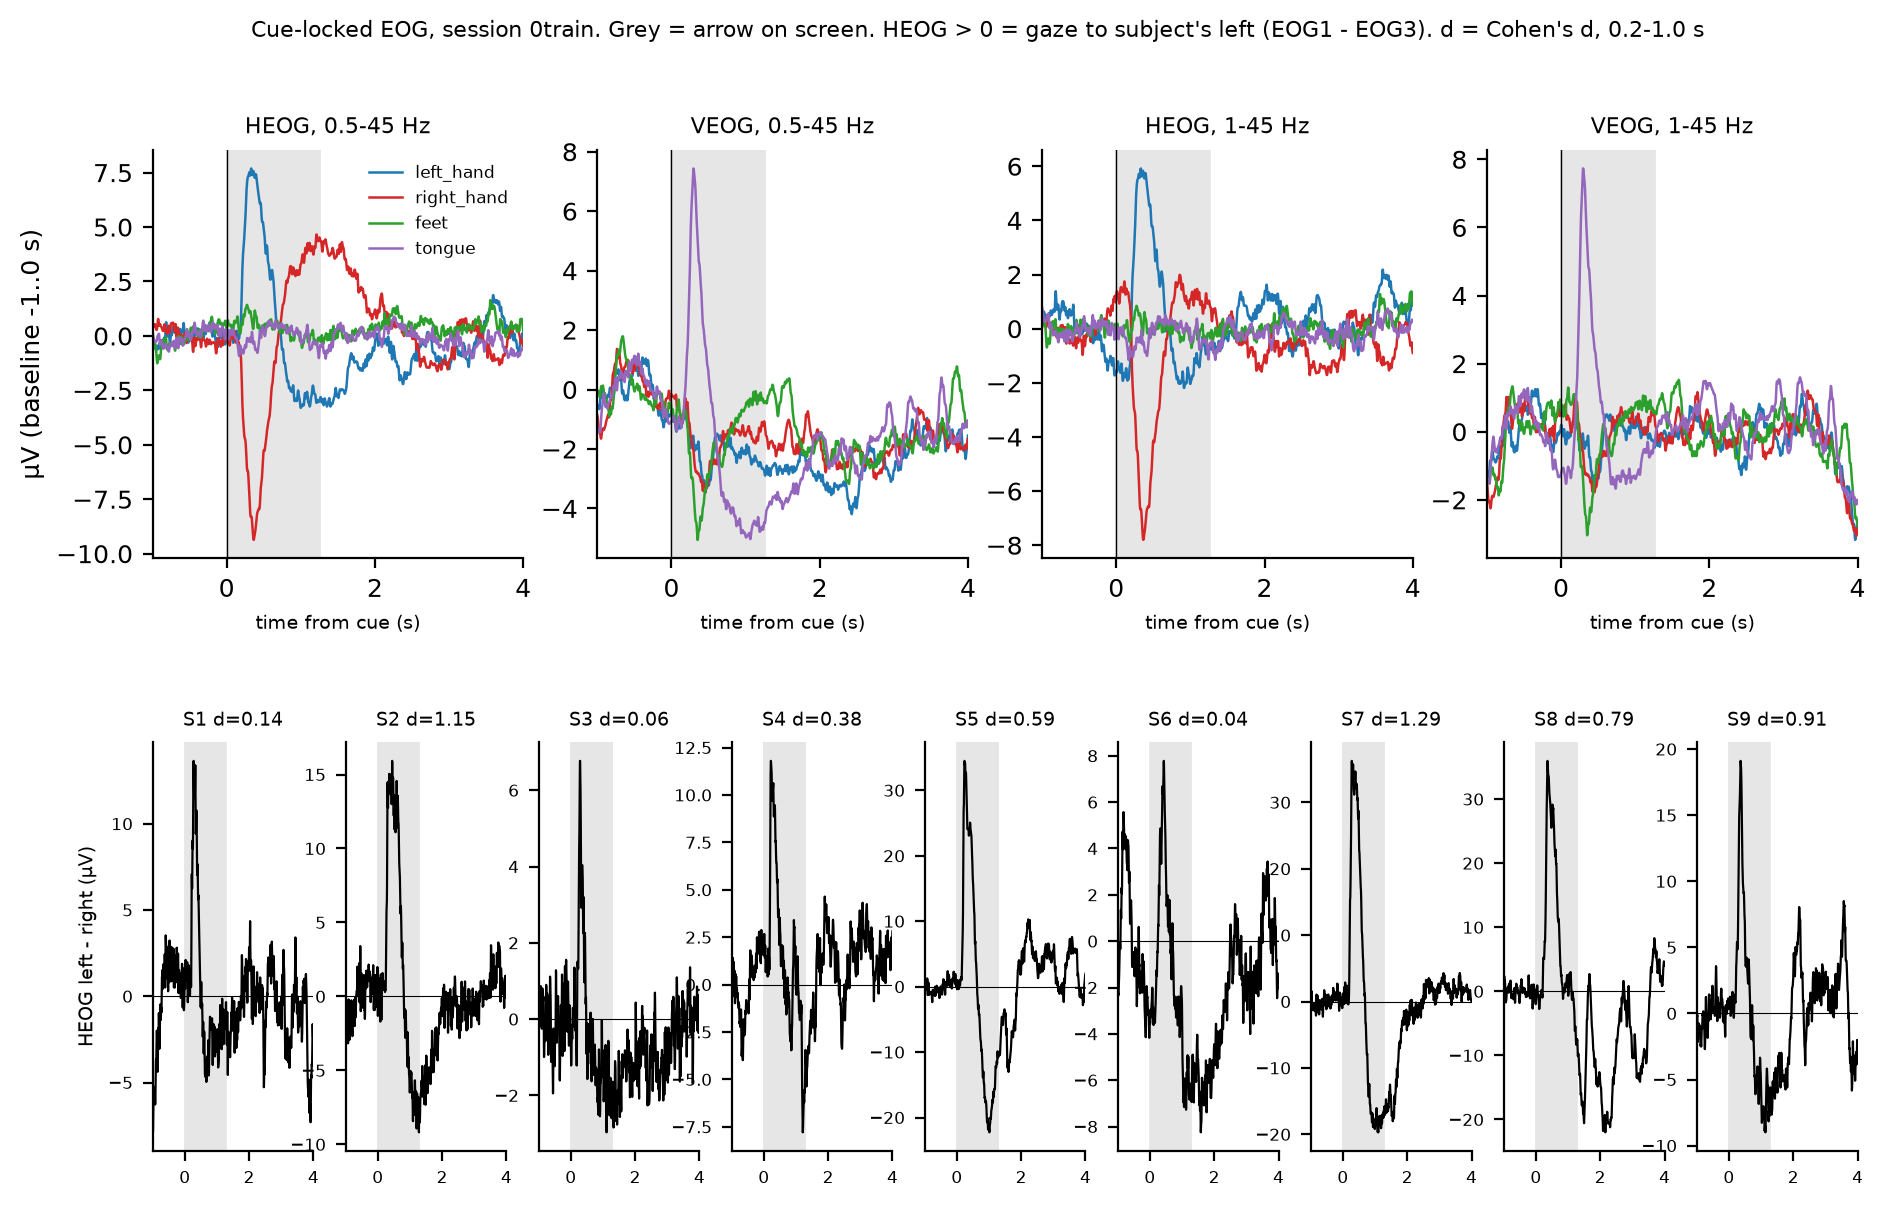
\includegraphics[width=0.95\textwidth]{fig_4c_eog_evoked_by_class.png}
\caption{Cue-locked EOG by class (session 0train). Top, grand averages of HEOG and VEOG. Bottom, HEOG difference between left and right cues per subject. Grey marks the 1.25~s arrow.}
\label{fig:eog}
\end{figure*}

\subsection{Features and classifiers}
All features are computed per trial and contain no learned parameter. Band power is the log of the mean Welch PSD (1~s Hamming segments with 50\% overlap) in the MI window, in delta 1--4, theta 4--8, mu 8--13, beta 13--30 and high 30--45~Hz bands. Amplitude features are baseline-corrected means in ten 100~ms bins from 0 to 1~s after the cue. Four feature sets form the main factor. \emph{eog\_only} uses EOG amplitude bins plus EOG delta and theta power (36 features). \emph{eeg\_all} uses all bands at all 22 EEG channels (110). \emph{eeg\_physio} uses mu and beta at C3, Cz, C4, FC3, FC4, CP3 and CP4 (14). \emph{eeg\_artifact\_prone} uses delta and high at Fz, FC1--FC4, C5 and C6 (14), the most frontal and lateral sites of this montage. The pipeline is a standard scaler followed by L2 logistic regression with $C=1$ and balanced class weights, or shrinkage LDA as a check. A nested leave-one-run-out search over $C$ changed the AUC by a median of \NestedDiff{}, so $C$ was fixed.

\subsection{Evaluation}
Each session was evaluated with leave-one-run-out cross-validation (6 folds, run as group). All learned steps were fitted inside the training folds, and an automated test checks that no training fold contains a test trial. Chance was estimated for every row by permuting labels within runs and repeating the same cross-validation, \NPermH{} times for the rows used by the H1 rule and fewer for the others because of the compute budget. Session 0train is primary and 1test is a replication. Training on 0train and testing on 1test gives an independent cross-session estimate. With nine subjects we used one-sided Wilcoxon signed-rank tests, for which the smallest attainable $p$ is 0.002, and Spearman correlations. The power of these tests is low and small effects can be missed.

\section{Results}
\textbf{H1 (\HoneVerdict{}).} EOG-only decoding of left versus right reached a median AUC of \AucEogNoneT{} in 0train and \AucEogNoneE{} in 1test (Fig.~\ref{fig:h1}). The median AUC minus 0.5 was \HoneDelta{} (IQR \HoneIqrLo{} to \HoneIqrHi{}, $W=\HoneW{}$, $p=\HoneP{}$), and \HoneAbove{} of \HoneN{} subjects exceeded the 95th percentile of their own null. H1 held in \RobHoneAll{} \RobHoneN{} robustness analyses (shrinkage LDA, session 1test, expert-flagged trials excluded, cross-session).

\begin{figure}[t]
\centering
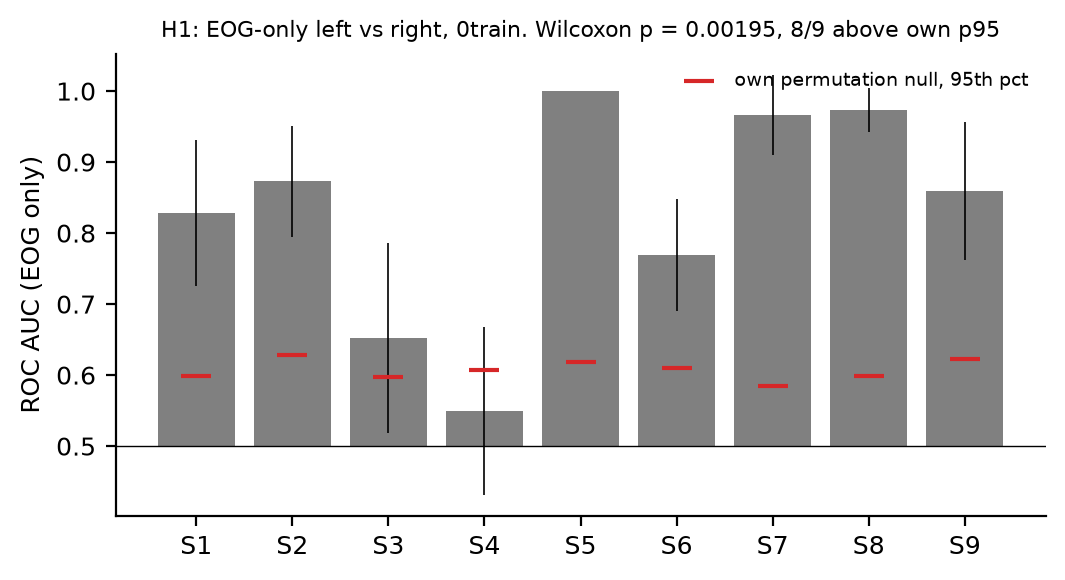
\includegraphics[width=\columnwidth]{fig_7a_eog_only_auc_vs_null.png}
\caption{H1. EOG-only AUC per subject with the 95th percentile of each subject's permutation null (red).}
\label{fig:h1}
\end{figure}

\textbf{H2 (\HtwoVerdict{}).} The \emph{eeg\_all} decoder reached a median AUC of \AucAllNoneT{} without cleaning, \AucAllRegT{} after regression and \AucAllIcaT{} after ICA. The paired drop was not different from zero (median \HtwoDeltaReg{}, $p=\HtwoPReg{}$ for regression, median \HtwoDeltaIca{}, $p=\HtwoPIca{}$ for ICA, both $p_{\text{Holm}}=\HtwoPholmIca{}$). The drop did not track the EOG-only AUC (Spearman $\rho=\HtwoRhoReg{}$ and \HtwoRhoIca{}). \RobHtwoAny{} of \RobHtwoN{} robustness tests supported H2.

\textbf{H3 (\HthreeVerdict{}).} After ICA the artifact-prone set did not lose more than the physiological set (median drops \HthreeDropProne{} and \HthreeDropPhysio{}, $p=\HthreeP{}$). Neither set lost AUC on average. The share of the \emph{eeg\_all} weight on central channels moved from \HthreeShareNone{}\% to \HthreeShareIca{}\% ($p=\HthreeShareP{}$), a change in the predicted direction that the test cannot distinguish from noise (Fig.~\ref{fig:weights}). The physiological set reached a median AUC of \AucPhysioNoneT{} and the artifact-prone set \AucProneNoneT{} (\AboveProneNoneT{} of 9 above chance).

\begin{figure*}[t]
\centering
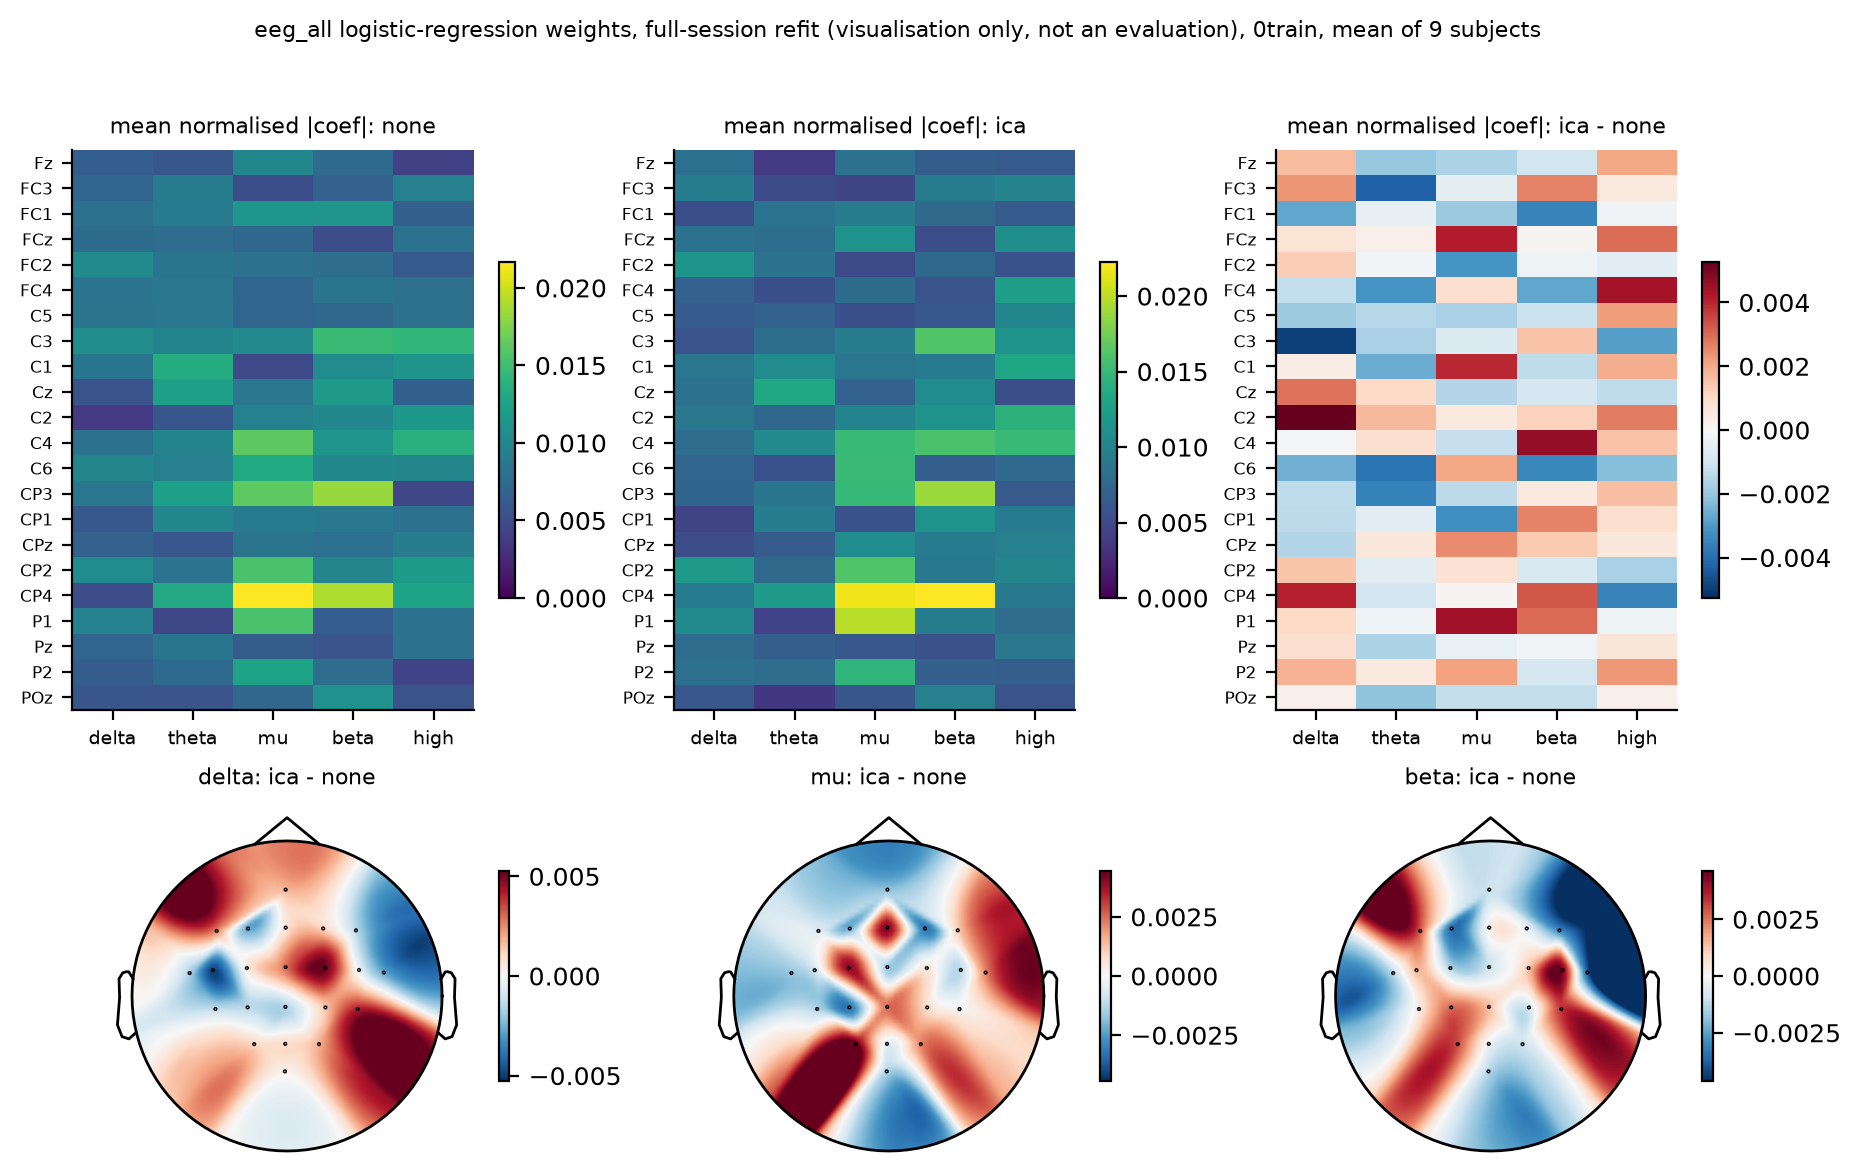
\includegraphics[width=0.9\textwidth]{fig_7c_feature_weights_before_after.png}
\caption{H3. Mean normalised weights of the \emph{eeg\_all} logistic regression (full-session refit, used for visualisation only) before and after ICA.}
\label{fig:weights}
\end{figure*}

\textbf{Four classes (secondary).} Multinomial logistic regression reached a median balanced accuracy of \BaccAllNone{} with \emph{eeg\_all} and \BaccEogNone{} with \emph{eog\_only} (chance 95th percentile about \BaccChance{}). The vertical arrows of the feet and tongue classes give the EOG its own class information, as Fig.~\ref{fig:eog} shows.

\textbf{Exploratory, not pre-registered.} The confound in Fig.~\ref{fig:eog} is a slow time-domain deflection, and every pre-registered EEG set uses band power. We therefore added one set of amplitude bins at Fz and FC1--FC4. Without cleaning it reached a median AUC of \ExAucNone{} (\ExAboveNone{} of 9 above chance). After regression it reached \ExAucReg{} and after ICA \ExAucIca{}. The median drop was small and not significant (\ExDeltaReg{} and \ExDeltaIca{}, Holm-corrected $p=\ExPholmReg{}$ and \ExPholmIca{}). The drop was however strongly related to the EOG-only AUC (Spearman $\rho=\ExRhoReg{}$, $p=\ExRhoPReg{}$ for regression and $\rho=\ExRhoIca{}$, $p=\ExRhoPIca{}$ for ICA). Subjects whose eyes carried the most class information lost the most frontal time-domain performance after cleaning. This analysis was chosen after seeing the H2 result and should be confirmed on new data.

\section{Discussion}
The arrow cue of dataset 2a produces a reflexive gaze shift toward the cued side in almost every subject, and the three EOG channels alone decode the hand class about as well as the full EEG. A decoder that uses the EOG, or time-domain features on frontal EEG, is therefore at risk of reporting eye movements as motor imagery. The standard band-power decoders tested here do not seem to rely on this signal. Removing it with two methods fitted on independent calibration data changed neither the AUC nor the weight maps in a measurable way. A likely reason is that the gaze shift is a brief, low-frequency event early in the trial, while the MI-window band power is dominated by mu and beta changes. The exploratory frontal amplitude result fits this reading only in part. Its median did not drop, but in subjects with large gaze shifts the time-domain decoder lost performance after cleaning in proportion to the EOG information.

Several limits apply. The study is offline and has nine subjects, so small cleaning effects cannot be excluded. EOG regression and ICA target ocular activity and do not remove EMG, which is the more likely contaminant for tongue imagery. Cleaning is incomplete at frontal sites, so the remaining part of the confound is not measured by our drops. Cleaning may also remove neural signal, although the physiological set did not lose AUC. The ICA threshold is semi-automatic, and its value and the score distribution are reported. A cue-locked eye movement is a reflex to the stimulus and not evidence that subjects tried to cheat. The S9 peak near 31~Hz over C4 differs strongly between classes ($p=\SNineHighP{}$) and is lateralised, which suggests that the high band is not purely artifactual.

For benchmark practice on 2a, results that use EOG channels, frontal time-domain features or windows overlapping the cue should report an EOG-only baseline next to their score. Our code reproduces every number in this report from a single notebook.

\section*{Appendix}
\textbf{AI-tool disclosure.} Claude Code (Anthropic) was used to write and run the analysis code, generate figures and draft this report under the direction of the team. All decisions and numbers were reviewed by the team and every number is generated from results/tables.

\textbf{Contributions.} See CONTRIBUTIONS.md and the git history.

\textbf{Supplementary tables.} stats\_robustness.csv, auc\_cross\_session.csv, auc\_expert\_artifacts\_excluded.csv and stats\_secondary\_4class.csv in results/tables.

\bibliographystyle{IEEEtran}
\bibliography{refs}
\end{document}
